% This LaTeX was auto-generated from MATLAB code.
% To make changes, update the MATLAB code and export to LaTeX again.

\documentclass{article}

\usepackage[utf8]{inputenc}
\usepackage[T1]{fontenc}
\usepackage{lmodern}
\usepackage{graphicx}
\usepackage{color}
\usepackage{listings}
\usepackage{hyperref}
\usepackage{amsmath}
\usepackage{amsfonts}
\usepackage{epstopdf}
\usepackage{matlab}

\sloppy
\epstopdfsetup{outdir=./}
\graphicspath{ {./ejercicio05_images/} }

\matlabmultipletitles

\begin{document}

\matlabtitle{Ejercicio N°5}


\begin{matlabcode}
clear;clc;
\end{matlabcode}

\begin{par}
\begin{flushleft}
Se definen simbólicas las variables
\end{flushleft}
\end{par}

\begin{matlabcode}
syms t vc1(t) vc2(t) il1(t) R1 R2 L1 C1 C2;
\end{matlabcode}

\begin{par}
\begin{flushleft}
Se plantean las ecuaciones y se obtienen las matrices de la forma generalizada
\end{flushleft}
\end{par}

\begin{matlabcode}
M=[C1 0 0; 0 C2 0; 0 0 L1]
\end{matlabcode}
\begin{matlabsymbolicoutput}
M = 
    $\displaystyle \left(\begin{array}{ccc}
C_1  & 0 & 0\\
0 & C_2  & 0\\
0 & 0 & L_1 
\end{array}\right)$
\end{matlabsymbolicoutput}
\begin{matlabcode}
N=[1/R1 0 1; 0 1/R2 -1; -1 1 0]
\end{matlabcode}
\begin{matlabsymbolicoutput}
N = 
    $\displaystyle \left(\begin{array}{ccc}
\frac{1}{R_1 } & 0 & 1\\
0 & \frac{1}{R_2 } & -1\\
-1 & 1 & 0
\end{array}\right)$
\end{matlabsymbolicoutput}
\begin{matlabcode}
u=[0;0;0]; 
\end{matlabcode}

\begin{par}
$$u=\left(\matrix{0\cr0\cr0}\right)$$
\end{par}

\begin{par}
\begin{flushleft}
Se expresan las matrices de la forma normalizada
\end{flushleft}
\end{par}

\begin{matlabcode}
A=-1.*(M\N)
\end{matlabcode}
\begin{matlabsymbolicoutput}
A = 
    $\displaystyle \left(\begin{array}{ccc}
-\frac{1}{C_1  R_1 } & 0 & -\frac{1}{C_1 }\\
0 & -\frac{1}{C_2  R_2 } & \frac{1}{C_2 }\\
\frac{1}{L_1 } & -\frac{1}{L_1 } & 0
\end{array}\right)$
\end{matlabsymbolicoutput}

\begin{par}
\begin{flushleft}
Se definen las variables de estado
\end{flushleft}
\end{par}

\begin{matlabcode}
x=[vc1;vc2;il1]
\end{matlabcode}
\begin{matlabsymbolicoutput}
x(t) = 
    $\displaystyle \left(\begin{array}{c}
{\textrm{vc}}_1 \left(t\right)\\
{\textrm{vc}}_2 \left(t\right)\\
{\textrm{il}}_1 \left(t\right)
\end{array}\right)$
\end{matlabsymbolicoutput}

\begin{par}
\begin{flushleft}
Expresando el sistema en forma diferencial
\end{flushleft}
\end{par}

\begin{matlabcode}
odes = diff(x) == A*x
\end{matlabcode}
\begin{matlabsymbolicoutput}
odes(t) = 
    $\displaystyle \left(\begin{array}{c}
\frac{\partial }{\partial t}\;{\textrm{vc}}_1 \left(t\right)=-\frac{{\textrm{il}}_1 \left(t\right)}{C_1 }-\frac{{\textrm{vc}}_1 \left(t\right)}{C_1  R_1 }\\
\frac{\partial }{\partial t}\;{\textrm{vc}}_2 \left(t\right)=\frac{{\textrm{il}}_1 \left(t\right)}{C_2 }-\frac{{\textrm{vc}}_2 \left(t\right)}{C_2  R_2 }\\
\frac{\partial }{\partial t}\;{\textrm{il}}_1 \left(t\right)=\frac{{\textrm{vc}}_1 \left(t\right)}{L_1 }-\frac{{\textrm{vc}}_2 \left(t\right)}{L_1 }
\end{array}\right)$
\end{matlabsymbolicoutput}

\begin{par}
\begin{flushleft}
Reemplazando los valores de los componentes
\end{flushleft}
\end{par}

\begin{matlabcode}
clear C1 C2 L1 R1 R2;
syms C1 C2;
R1=1;R2=1;C1=1;C2=1;L1=2;
A=subs(A);
odes = diff(x) == A*x;
\end{matlabcode}

\begin{par}
\begin{flushleft}
Definiendo las condiciones iniciales y tiempo de simulacion
\end{flushleft}
\end{par}

\begin{matlabcode}
vc01=1/2;
vc02=1/2;
il0=1/2;
ti=0;
tf=10;
Xant=[vc01;vc02;il0];
constantes=x(0)==Xant;
[vc1Sol(t), vc2Sol(t), il1Sol(t)] = dsolve(odes,constantes);
\end{matlabcode}

\matlabtitle{Tensión sobre R2}

\begin{matlabcode}
simplify(vc2Sol(t))
\end{matlabcode}
\begin{matlabsymbolicoutput}
ans = 
    $\displaystyle \frac{e^{-t} }{2}-\frac{\sqrt{3} \sin \left(\frac{\sqrt{3} t}{2}\right)}{3 \sqrt{e^t }}$
\end{matlabsymbolicoutput}


\matlabtitle{Respuesta temporal vR2(t)}

\begin{matlabcode}
clf;
fplot(vc2Sol,[ti,tf],'-g')
title('Respuesta temporal')
xlabel('tiempo [s]')
ylabel('Voltaje [V]')
legend({'Voltaje R2'})
\end{matlabcode}
\begin{center}
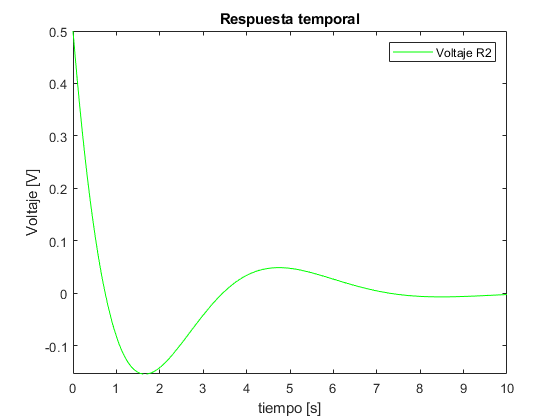
\includegraphics[width=\maxwidth{56.196688409433015em}]{figure_0_05}
\end{center}

\end{document}
